\documentclass[12pt]{article}
\usepackage[utf8]{inputenc}
\usepackage{graphicx}
\usepackage{xcolor}
\usepackage{tikz}
\usetikzlibrary{shapes.geometric, arrows, positioning}
\usepackage{listings}
\usepackage{geometry}
\geometry{a4paper, margin=1in}

\definecolor{codebg}{rgb}{0.95,0.95,0.95}
\lstset{
    backgroundcolor=\color{codebg},
    basicstyle=\ttfamily\small,
    breaklines=true,
    frame=single
}

% Define colors for diagrams
\definecolor{frontend}{RGB}{255,200,200}
\definecolor{backend}{RGB}{200,220,255}
\definecolor{database}{RGB}{200,255,200}

\title{\textbf{Pharmacy Management Application} \\ Database \& Connection Explanation for Beginners}
\author{A Simple Guide for Kids and Beginners}
\date{\today}

\begin{document}

\maketitle
\newpage

\tableofcontents
\newpage

\section{What is a Database? 🗄️}

Imagine you have a magical notebook that:
\begin{itemize}
    \item Never runs out of pages
    \item Can find any information instantly
    \item Never loses any information
    \item Can be read by computers
\end{itemize}

That's what a database is! It's a special place on the computer where we store all our important information.

\subsection{Our Database - MongoDB}

Our pharmacy application uses MongoDB, which is like having many organized boxes:
\begin{itemize}
    \item One box for all customer information
    \item One box for all medicine information
    \item One box for all orders
    \item One box for all prescriptions
\end{itemize}

In MongoDB, these "boxes" are called \textbf{Collections}, and each item in a box is called a \textbf{Document}.

\section{What Information Do We Store?}

\subsection{Users Collection - Customer Information Box 👤}

Every customer who signs up gets their information saved here:

\begin{center}
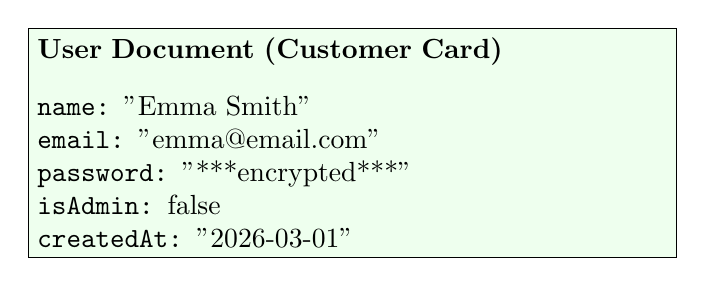
\begin{tikzpicture}[node distance=2cm]
    \node[draw, rectangle, fill=database!30, text width=8cm, align=left] {
        \textbf{User Document (Customer Card)} \\[0.3cm]
        \texttt{name:} "Emma Smith" \\
        \texttt{email:} "emma@email.com" \\
        \texttt{password:} "***encrypted***" \\
        \texttt{isAdmin:} false \\
        \texttt{createdAt:} "2026-03-01"
    };
\end{tikzpicture}
\end{center}

\textbf{Think of it like:} A membership card for each customer!
\begin{itemize}
    \item \textbf{name:} The customer's name
    \item \textbf{email:} Their email address (must be unique - no two people can use the same email!)
    \item \textbf{password:} Their secret password (stored in scrambled form so nobody can read it!)
    \item \textbf{isAdmin:} True if they're a manager, false if they're a customer
    \item \textbf{createdAt:} When they signed up
\end{itemize}

\subsection{Products Collection - Medicine Information Box 💊}

Every medicine in our pharmacy is stored here:

\begin{center}
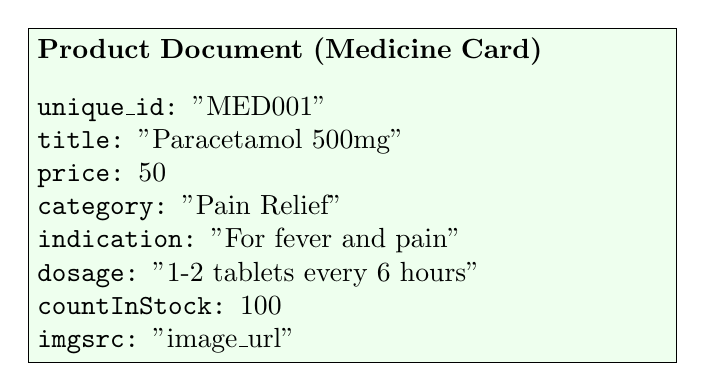
\begin{tikzpicture}[node distance=2cm]
    \node[draw, rectangle, fill=database!30, text width=8cm, align=left] {
        \textbf{Product Document (Medicine Card)} \\[0.3cm]
        \texttt{unique\_id:} "MED001" \\
        \texttt{title:} "Paracetamol 500mg" \\
        \texttt{price:} 50 \\
        \texttt{category:} "Pain Relief" \\
        \texttt{indication:} "For fever and pain" \\
        \texttt{dosage:} "1-2 tablets every 6 hours" \\
        \texttt{countInStock:} 100 \\
        \texttt{imgsrc:} "image\_url"
    };
\end{tikzpicture}
\end{center}

\textbf{Think of it like:} A detailed label on each medicine bottle!

\subsection{Orders Collection - Shopping Receipt Box 🛒}

When someone buys medicine, we save the order here:

\begin{center}
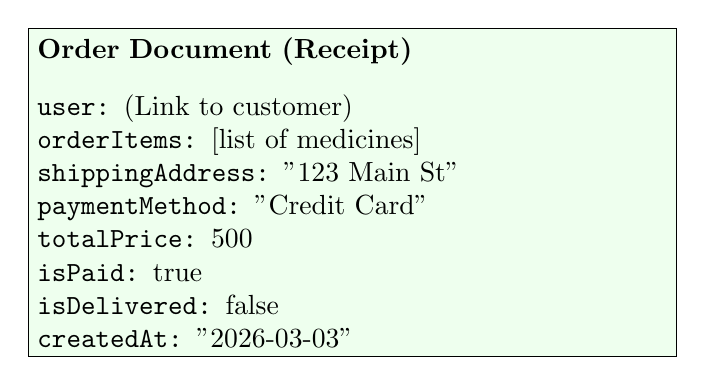
\begin{tikzpicture}[node distance=2cm]
    \node[draw, rectangle, fill=database!30, text width=8cm, align=left] {
        \textbf{Order Document (Receipt)} \\[0.3cm]
        \texttt{user:} (Link to customer) \\
        \texttt{orderItems:} [list of medicines] \\
        \texttt{shippingAddress:} "123 Main St" \\
        \texttt{paymentMethod:} "Credit Card" \\
        \texttt{totalPrice:} 500 \\
        \texttt{isPaid:} true \\
        \texttt{isDelivered:} false \\
        \texttt{createdAt:} "2026-03-03"
    };
\end{tikzpicture}
\end{center}

\textbf{Think of it like:} A receipt you get after shopping!

\subsection{Contact Collection - Message Box 📧}

When someone sends us a message through the contact form:

\begin{center}
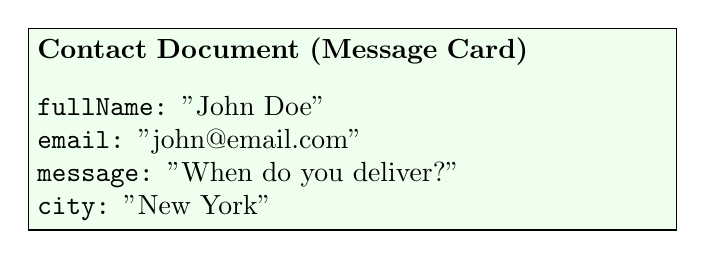
\begin{tikzpicture}[node distance=2cm]
    \node[draw, rectangle, fill=database!30, text width=8cm, align=left] {
        \textbf{Contact Document (Message Card)} \\[0.3cm]
        \texttt{fullName:} "John Doe" \\
        \texttt{email:} "john@email.com" \\
        \texttt{message:} "When do you deliver?" \\
        \texttt{city:} "New York"
    };
\end{tikzpicture}
\end{center}

\section{How Frontend Connects to Backend 🔗}

\subsection{The Three-Part Team}

Our pharmacy application works like a team of three friends:

\begin{center}
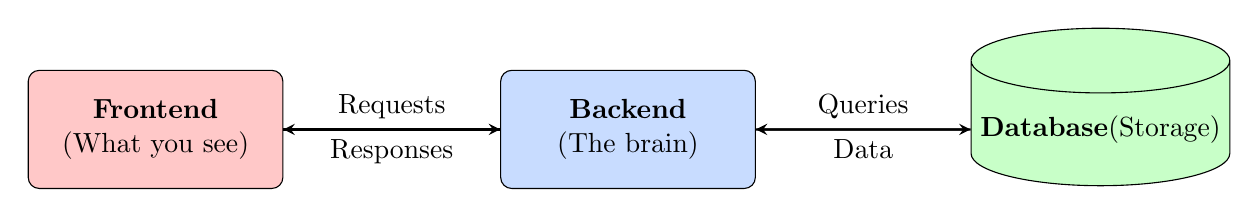
\begin{tikzpicture}[node distance=3cm, auto]
    % Define styles
    \tikzstyle{frontend} = [rectangle, rounded corners, minimum width=3cm, minimum height=1.5cm, text centered, draw=black, fill=frontend, text width=3cm]
    \tikzstyle{backend} = [rectangle, rounded corners, minimum width=3cm, minimum height=1.5cm, text centered, draw=black, fill=backend, text width=3cm]
    \tikzstyle{database} = [cylinder, shape border rotate=90, aspect=0.25, minimum width=3cm, minimum height=2cm, draw=black, fill=database, text centered]
    \tikzstyle{arrow} = [thick,->,>=stealth]
    
    % Nodes
    \node (frontend) [frontend] {\textbf{Frontend} \\ (What you see)};
    \node (backend) [backend, right of=frontend, xshift=3cm] {\textbf{Backend} \\ (The brain)};
    \node (db) [database, right of=backend, xshift=3cm] {\textbf{Database} \\ (Storage)};
    
    % Arrows
    \draw [arrow] (frontend) -- node[anchor=south] {Requests} (backend);
    \draw [arrow] (backend) -- node[anchor=north] {Responses} (frontend);
    \draw [arrow] (backend) -- node[anchor=south] {Queries} (db);
    \draw [arrow] (db) -- node[anchor=north] {Data} (backend);
\end{tikzpicture}
\end{center}

\subsection{The Connection Journey}

Let's follow what happens when someone wants to see all medicines:

\begin{center}
\begin{tikzpicture}[node distance=2.5cm, auto]
    \tikzstyle{step} = [rectangle, rounded corners, minimum width=6cm, minimum height=1cm, text centered, draw=black, fill=blue!20]
    
    \node (step1) [step] {1. Customer clicks "View Products"};
    \node (step2) [step, below of=step1] {2. Frontend sends request to Backend};
    \node (step3) [step, below of=step2] {3. Backend asks Database for products};
    \node (step4) [step, below of=step3] {4. Database sends product list back};
    \node (step5) [step, below of=step4] {5. Backend sends data to Frontend};
    \node (step6) [step, below of=step5] {6. Frontend shows products on screen};
    
    \draw [arrow] (step1) -- (step2);
    \draw [arrow] (step2) -- (step3);
    \draw [arrow] (step3) -- (step4);
    \draw [arrow] (step4) -- (step5);
    \draw [arrow] (step5) -- (step6);
\end{tikzpicture}
\end{center}

\section{Important Connection Files}

\subsection{Database Connection File - db.js}

\textbf{Location:} \texttt{backend/config/db.js}

This file is like a phone that calls the database and says "Hello! Let's connect!"

\begin{lstlisting}[language=JavaScript]
// This function connects us to MongoDB
const connectDB = async () => {
  try {
    // Try to connect using the database address
    await mongoose.connect(process.env.MONGO_URI);
    console.log("Database connected successfully!");
  } catch (error) {
    console.log("Connection failed!");
  }
};
\end{lstlisting}

\textbf{Simple explanation:}
\begin{itemize}
    \item It tries to connect to MongoDB
    \item If successful: "Yay! Connected!"
    \item If failed: "Oh no! Connection failed!"
\end{itemize}

\subsection{Frontend Request Files - Actions}

\textbf{Location:} \texttt{frontend/src/redux/actions/}

These files send requests from frontend to backend.

\subsubsection{Example: userActions.js}

When someone tries to login:

\begin{lstlisting}[language=JavaScript]
// Send login request to backend
const { data } = await axios.post(
  "/api/users/login",
  { email, password }
);
\end{lstlisting}

\textbf{What's happening:}
\begin{enumerate}
    \item Frontend collects email and password
    \item Sends them to backend at address \texttt{/api/users/login}
    \item Waits for backend to check if they're correct
    \item Gets back user information if login successful
\end{enumerate}

\section{The Complete Data Flow}

\subsection{Example 1: Customer Registration}

\begin{center}
\begin{tikzpicture}[node distance=1.8cm, every node/.style={font=\small}]
    \tikzstyle{box} = [rectangle, rounded corners, minimum width=7cm, minimum height=0.8cm, text centered, draw=black]
    
    \node (a) [box, fill=frontend] {1. SignUpScreen.js - Customer fills registration form};
    \node (b) [box, below of=a, fill=frontend] {2. userActions.js - Sends data to /api/users};
    \node (c) [box, below of=b, fill=backend] {3. userRoutes.js - Receives request};
    \node (d) [box, below of=c, fill=backend] {4. userControllers.js - Creates new user};
    \node (e) [box, below of=d, fill=database] {5. User.js model - Saves to MongoDB};
    \node (f) [box, below of=e, fill=backend] {6. Backend sends success response};
    \node (g) [box, below of=f, fill=frontend] {7. Frontend receives confirmation};
    \node (h) [box, below of=g, fill=frontend] {8. Customer sees "Account Created!" message};
    
    \draw [arrow] (a) -- (b);
    \draw [arrow] (b) -- (c);
    \draw [arrow] (c) -- (d);
    \draw [arrow] (d) -- (e);
    \draw [arrow] (e) -- (f);
    \draw [arrow] (f) -- (g);
    \draw [arrow] (g) -- (h);
\end{tikzpicture}
\end{center}

\subsection{Example 2: Viewing All Products}

\begin{center}
\begin{tikzpicture}[node distance=1.8cm, every node/.style={font=\small}]
    \tikzstyle{box} = [rectangle, rounded corners, minimum width=7cm, minimum height=0.8cm, text centered, draw=black]
    
    \node (a) [box, fill=frontend] {1. AllProductsScreen.js - Page loads};
    \node (b) [box, below of=a, fill=frontend] {2. productActions.js - Requests all products};
    \node (c) [box, below of=b, fill=backend] {3. productRoutes.js - Routes to controller};
    \node (d) [box, below of=c, fill=backend] {4. productControllers.js - Queries database};
    \node (e) [box, below of=d, fill=database] {5. Product.js model - Gets all products};
    \node (f) [box, below of=e, fill=backend] {6. Backend sends product list};
    \node (g) [box, below of=f, fill=frontend] {7. Frontend stores in Redux};
    \node (h) [box, below of=g, fill=frontend] {8. Products displayed on screen};
    
    \draw [arrow] (a) -- (b);
    \draw [arrow] (b) -- (c);
    \draw [arrow] (c) -- (d);
    \draw [arrow] (d) -- (e);
    \draw [arrow] (e) -- (f);
    \draw [arrow] (f) -- (g);
    \draw [arrow] (g) -- (h);
\end{tikzpicture}
\end{center}

\section{Key Directories and Their Roles}

\subsection{Frontend Side}

\begin{center}
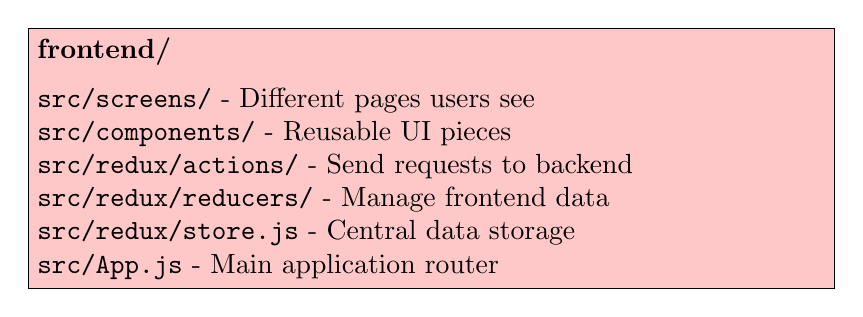
\begin{tikzpicture}[node distance=2.5cm]
    \node[draw, rectangle, fill=frontend, text width=10cm, align=left] {
        \textbf{frontend/} \\[0.2cm]
        \texttt{src/screens/} - Different pages users see \\
        \texttt{src/components/} - Reusable UI pieces \\
        \texttt{src/redux/actions/} - Send requests to backend \\
        \texttt{src/redux/reducers/} - Manage frontend data \\
        \texttt{src/redux/store.js} - Central data storage \\
        \texttt{src/App.js} - Main application router
    };
\end{tikzpicture}
\end{center}

\subsection{Backend Side}

\begin{center}
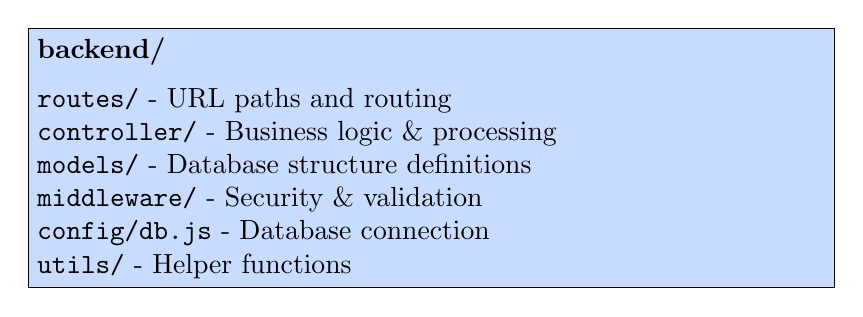
\begin{tikzpicture}[node distance=2.5cm]
    \node[draw, rectangle, fill=backend, text width=10cm, align=left] {
        \textbf{backend/} \\[0.2cm]
        \texttt{routes/} - URL paths and routing \\
        \texttt{controller/} - Business logic \& processing \\
        \texttt{models/} - Database structure definitions \\
        \texttt{middleware/} - Security \& validation \\
        \texttt{config/db.js} - Database connection \\
        \texttt{utils/} - Helper functions
    };
\end{tikzpicture}
\end{center}

\subsection{Root Level}

\begin{center}
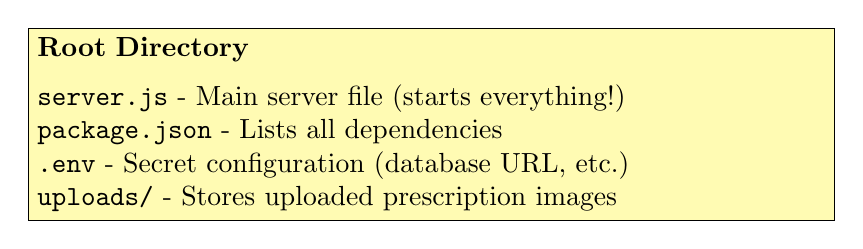
\begin{tikzpicture}[node distance=2.5cm]
    \node[draw, rectangle, fill=yellow!30, text width=10cm, align=left] {
        \textbf{Root Directory} \\[0.2cm]
        \texttt{server.js} - Main server file (starts everything!) \\
        \texttt{package.json} - Lists all dependencies \\
        \texttt{.env} - Secret configuration (database URL, etc.) \\
        \texttt{uploads/} - Stores uploaded prescription images
    };
\end{tikzpicture}
\end{center}

\section{URL Patterns - The Address System}

Think of URLs like house addresses! Each part of our application has an address:

\subsection{Product-Related URLs}

\begin{itemize}
    \item \texttt{GET /api/products} - Get all medicines
    \item \texttt{GET /api/products/:id} - Get one specific medicine
    \item \texttt{POST /api/products} - Add new medicine (admin only)
    \item \texttt{PUT /api/products/:id} - Update a medicine
    \item \texttt{DELETE /api/products/:id} - Remove a medicine
\end{itemize}

\subsection{User-Related URLs}

\begin{itemize}
    \item \texttt{POST /api/users} - Register new user
    \item \texttt{POST /api/users/login} - Login
    \item \texttt{GET /api/users/profile} - Get user profile
    \item \texttt{PUT /api/users/profile} - Update profile
\end{itemize}

\subsection{Order-Related URLs}

\begin{itemize}
    \item \texttt{POST /api/orders} - Create new order
    \item \texttt{GET /api/orders/myorders} - Get my orders
    \item \texttt{GET /api/orders/:id} - Get one specific order
\end{itemize}

\section{How Data Travels - A Real Example}

Let's follow what happens when Emma wants to buy Paracetamol:

\subsection{Step-by-Step Journey}

\begin{enumerate}
    \item \textbf{Emma opens the website}
    \begin{itemize}
        \item Browser loads \texttt{App.js}
        \item Shows \texttt{HomeScreen.js}
    \end{itemize}
    
    \item \textbf{Emma clicks "View All Products"}
    \begin{itemize}
        \item \texttt{App.js} shows \texttt{AllProductsScreen.js}
        \item This screen calls \texttt{productActions.js}
    \end{itemize}
    
    \item \textbf{Frontend requests products}
    \begin{itemize}
        \item \texttt{productActions.js} sends GET request to \texttt{/api/products}
        \item Request travels over the internet to backend
    \end{itemize}
    
    \item \textbf{Backend receives request}
    \begin{itemize}
        \item \texttt{server.js} receives request
        \item Routes it to \texttt{productRoutes.js}
        \item Calls \texttt{productControllers.js}
    \end{itemize}
    
    \item \textbf{Getting data from database}
    \begin{itemize}
        \item Controller uses \texttt{Product.js} model
        \item Queries MongoDB for all products
        \item MongoDB searches its Products collection
    \end{itemize}
    
    \item \textbf{Sending data back}
    \begin{itemize}
        \item Database returns product list
        \item Controller sends list to frontend
    \end{itemize}
    
    \item \textbf{Frontend receives data}
    \begin{itemize}
        \item Data stored in Redux store
        \item \texttt{AllProductsScreen.js} reads from store
        \item Displays products using \texttt{Product.js} component
    \end{itemize}
    
    \item \textbf{Emma sees all medicines!}
    \begin{itemize}
        \item Each medicine shown as a card
        \item Shows image, name, price
        \item "Add to Cart" button available
    \end{itemize}
\end{enumerate}

\section{Security Features 🔒}

\subsection{Password Protection}

When Emma creates an account:
\begin{enumerate}
    \item She types password: "mypassword123"
    \item Backend receives it
    \item \texttt{User.js} model scrambles it using bcrypt
    \item Saved as: "\$2a\$10\$N9qo8u..." (unreadable!)
    \item When logging in, backend compares scrambled versions
\end{enumerate}

\subsection{Authentication Tokens}

After login:
\begin{enumerate}
    \item Backend creates a special token (like a temporary ID card)
    \item Frontend stores it in browser
    \item For every request, frontend sends this token
    \item \texttt{authMiddleware.js} checks if token is valid
    \item Only valid tokens can access protected routes
\end{enumerate}

\section{Summary - The Big Picture}

\subsection{Three Main Parts Working Together}

\begin{center}
\begin{tikzpicture}[node distance=3cm]
    \node[draw, circle, fill=frontend, minimum size=3cm, align=center] (fe) {\textbf{Frontend} \\ User Interface \\ React App};
    \node[draw, circle, fill=backend, minimum size=3cm, align=center, right of=fe, xshift=3cm] (be) {\textbf{Backend} \\ Business Logic \\ Express Server};
    \node[draw, circle, fill=database, minimum size=3cm, align=center, below of=fe, yshift=-1cm, xshift=3cm] (db) {\textbf{Database} \\ Data Storage \\ MongoDB};
    
    \draw[arrow, bend right, thick] (fe) to node[above] {HTTP Requests} (be);
    \draw[arrow, bend right, thick] (be) to node[below] {JSON Response} (fe);
    \draw[arrow, bend left, thick] (be) to node[right] {Queries} (db);
    \draw[arrow, bend left, thick] (db) to node[left] {Data} (be);
\end{tikzpicture}
\end{center}

\subsection{Remember These Key Points}

\begin{itemize}
    \item \textbf{Frontend} talks to \textbf{Backend} using URLs (like \texttt{/api/products})
    \item \textbf{Backend} talks to \textbf{Database} using models (like \texttt{Product.js})
    \item Data flows: Frontend → Backend → Database → Backend → Frontend
    \item Each part has a specific job and they work as a team!
    \item Files are organized in folders by their purpose
    \item Security is important - passwords are scrambled, tokens are checked
\end{itemize}

\subsection{The Magic of APIs}

API stands for "Application Programming Interface" - but think of it as a \textbf{waiter in a restaurant}:
\begin{itemize}
    \item You (Frontend) tell the waiter (API) what you want
    \item Waiter goes to the kitchen (Backend/Database)
    \item Kitchen prepares your order
    \item Waiter brings it back to you
    \item You never have to go to the kitchen yourself!
\end{itemize}

Our URLs like \texttt{/api/products} are the menu items you can order!

\section{Conclusion}

You now understand:
\begin{itemize}
    \item What a database is and what information we store
    \item How frontend, backend, and database work together
    \item The journey of data from screen to database and back
    \item Important files and their roles
    \item How the whole system connects together
\end{itemize}

\textbf{Remember:} Building an application is like building with LEGO blocks - many small pieces working together to create something amazing!

\end{document}
